% !TEX TS-program = lualatex
% !TEX encoding = UTF-8 Unicode
% !BIB program = biber 

\documentclass[article, 12pt, oneside]{memoir}
\usepackage[dvipsnames]{xcolor}
\usepackage{amsmath, amssymb}
\usepackage{xspace}
\usepackage{hyperref}
\usepackage{longtable}

\usepackage[tracking, protrusion]{microtype}

\usepackage{fontspec}
\setmainfont{Alegreya}
\setsansfont{Alegreya Sans}
\setmonofont[Scale=MatchLowercase]{Menlo}
\linespread{1.1}

\hypersetup{
  unicode=true,
  linktocpage=true,
  linkcolor=NavyBlue,
  colorlinks=true,
  urlcolor=NavyBlue,
  citecolor=RoyalBlue,
  breaklinks=true,
}

\def\sectionautorefname{§}
\def\subsectionautorefname{§}

\renewcommand{\bf}{\bfseries}
\renewcommand{\it}{\itshape}

% ======================================================================
% Graphics
% ======================================================================
\usepackage{graphicx,grffile}
\makeatletter
\def\maxwidth{\ifdim\Gin@nat@width>\linewidth\linewidth\else\Gin@nat@width\fi}
\def\maxheight{\ifdim\Gin@nat@height>\textheight\textheight\else\Gin@nat@height\fi}
\makeatother
% Scale images if necessary, so that they will not overflow the page
% margins by default, and it is still possible to overwrite the defaults
% using explicit options in \includegraphics[width, height, ...]{}
\setkeys{Gin}{width=\maxwidth,height=\maxheight,keepaspectratio}
% ======================================================================
% Memoir layout and formatting specifications
% ======================================================================
%\setlrmarginsandblock{1.91in}{*}{*}
%\setulmarginsandblock{1in}{*}{*}
\setsecnumdepth{subsection}
\settocdepth{subsection}
\setsecheadstyle{\color{Maroon}\large\sffamily\bfseries}
\setsubsecheadstyle{\bfseries}
\setparaheadstyle{\bfseries\sffamily}
\tightlists

\counterwithout{section}{chapter}
\captionstyle[\centering]{\sffamily\small}
\captionnamefont{\color{Maroon}\sffamily\small}
\captionwidth{0.95\textwidth}
\changecaptionwidth


\checkandfixthelayout


\title{Month 3 Report:\\Description of Prototype System}
\author{\href{https://ml4ai.github.io/automates/team/}{The AutoMATES Team}}
\date{2019-02-01}

\begin{document}
\maketitle
\tableofcontents*

\bigskip
\bigskip

\noindent \emph{Note: This PDF has been automatically generated from a web
  version, available here:}

  {
  \small
\noindent \url{https://ml4ai.github.io/automates/documentation/reports/m3_report_prototype_system}
}

\hypertarget{overview}{%
\section{Overview}\label{overview}}

In this report, the AutoMATES team describes the development work done
in the past two months on the AutoMATES prototype system. No changes
have been made to the overall architecture and design, but significant
progress has been made in each of the architecture components introduced
in the
\href{https://ml4ai.github.io/automates/documentation/reports/m1_architecture_report/}{Month
1 Report}. We are on track for successfully achieving our Phase 1 goals
for the prototype. Among the highlights for this phase are the
following: 

\begin{itemize}
\tightlist
\item
  Deployment of a demonstration web application of the program
  analysis-to-function network translation translation.
\item
  Extension of the GrFN representation to represent namespaces in
  identifiers, for handling multi-file and multi-module systems.
\item
  Extensions of the Fortran program analysis module for handling Fortran
  I/O, Modules, open-ended loops, and arrays.
\item
  Development of the text reading pipeline for converting PDFs to text,
  extracting quantities and their domains, and a start to developing
  grammars for extracting variables and associating them with values.
\item
  Development of the equation detection and parsing pipeline as well as
  collecting the enormous arXiv PDF and TeX source corpus.
\item
  Development of an algorithm to identify structural overlap between two
  models, through the identification of the Forward Influence Blanket.
\item
  Improving the code summarization training corpus by expanding it
  dramatically, as well as progress in improving the embedding model for
  code summary generation.
\end{itemize}

All code supporting the contributions reported here is available in the
\href{https://github.com/ml4ai/automates}{AutoMATES} and
\href{https://github.com/ml4ai/delphi/}{Delphi} Github repositories.

% \begin{center}\rule{0.5\linewidth}{\linethickness}\end{center}

\hypertarget{demo-webapp}{%
\section{Demo Webapp}\label{demo-webapp}}

A demo of the current version of the prototype system is now live - you
can \href{http://vanga.sista.arizona.edu/automates}{try it
out here}!

\begin{figure}
\centering
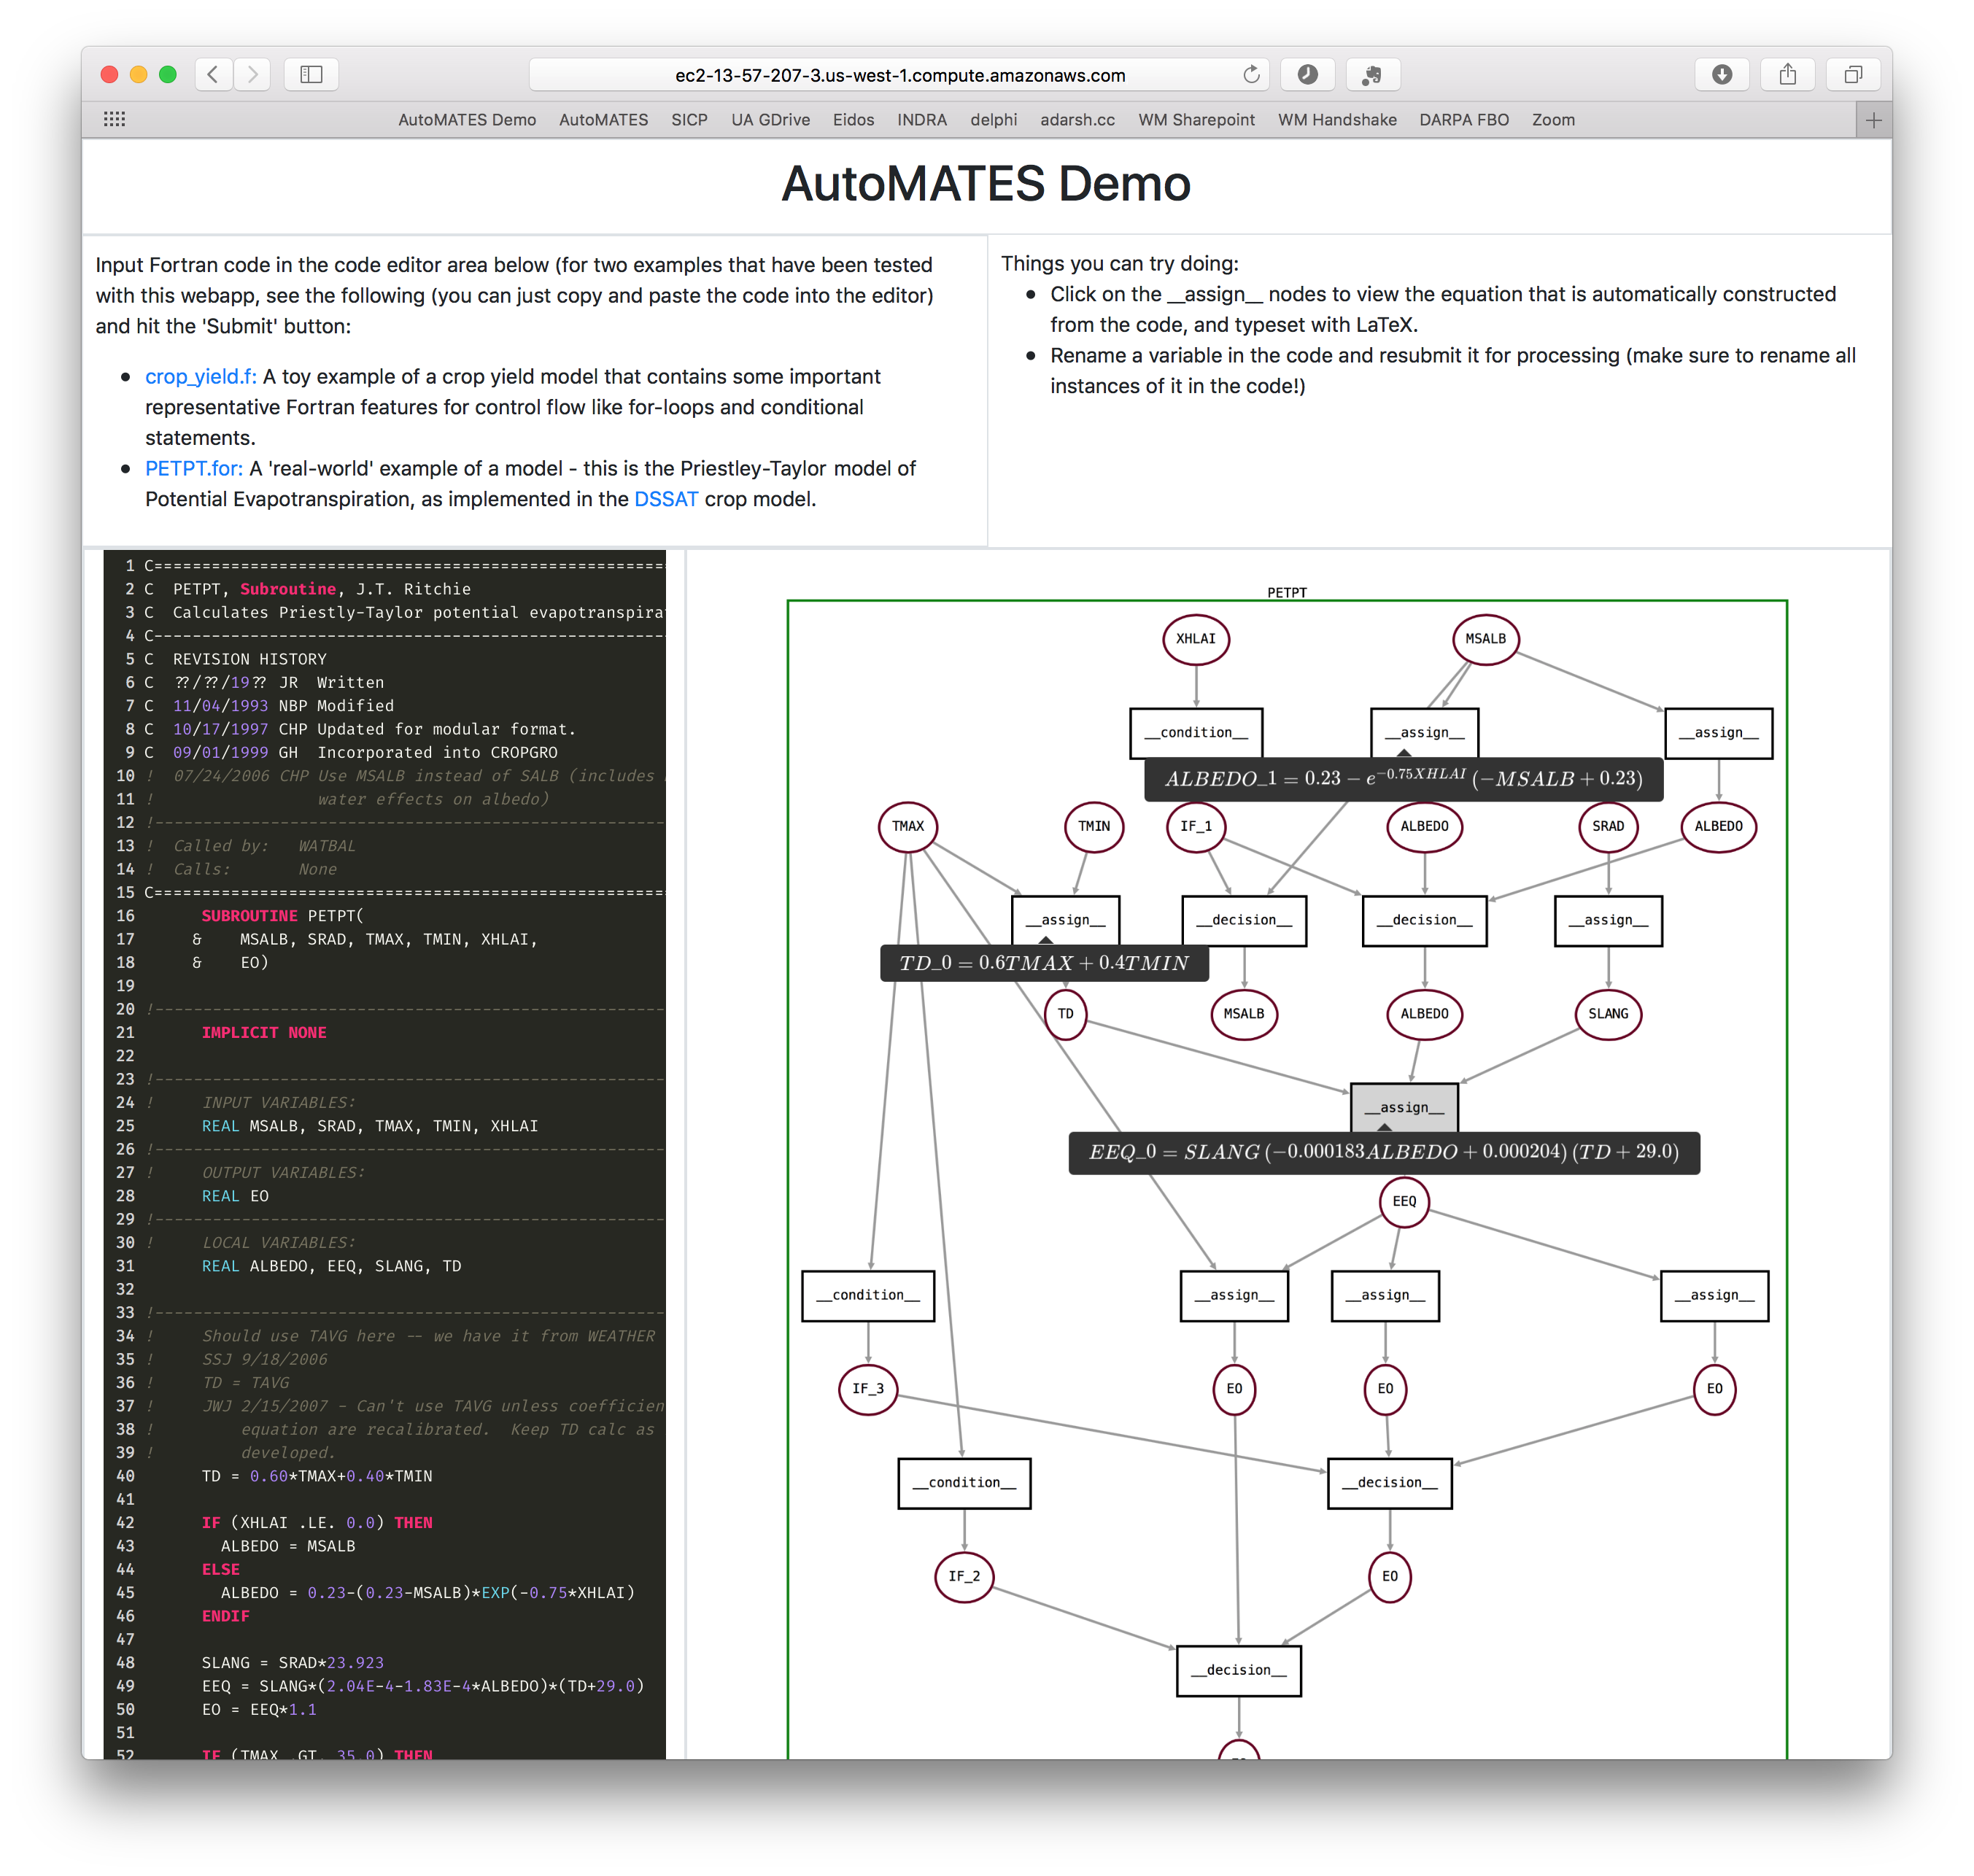
\includegraphics{figs/webapp_screenshot.png}
\caption{Screenshot of AutoMATES demo webapp.\label{fig:webapp}}
\end{figure}

When Fortran source code is submitted to the demo, it is processed by
the Program Analysis (\texttt{for2py}) pipeline, generating both (1)
equivalent target executable Python internal representation and (2)
matching GrFN specification representation. The GrFN specification is
then rendered as a function network graph that you can interact with.

Currently, the demo has been only been tested with a limited number of
programs, so we encourage users as of now to experiment by modifying the
two suggested examples on the page, rather than trying to process
arbitrary Fortran programs.

Clicking on the \texttt{\_\_assign\_\_} nodes in the rendered GrFN
function network graph yields a LaTeX representation of the equation
corresponding to the assign statement. This equation is constructed from
the Python source represented using
\href{https://www.sympy.org}{\texttt{SymPy}}, and will facilitate the
linkage to equations extracted from papers using the equation parsing
module.

For example, the screenshot in Figure~\ref{fig:webapp} shows the analysis of the
Priestley-Taylor method of calculating potential evapotranspiration, as
implemented in DSSAT. Three of the \texttt{\_\_assign\_\_} functions
have been clicked, showing tooltips with black backgrounds containing
some of the equations involved in this calculation - these very
equations can be found on page 46 of the book
\href{https://link-springer-com.ezproxy2.library.arizona.edu/book/10.1007\%2F978-94-017-3624-4}{Understanding
Options for Agricultural Production} (reproduced in Figure~\ref{fig:uoap-book} - the equations
matching the ones in the screenshot of the webapp are highlighted with
maroon borders).

% \begin{center}\rule{0.5\linewidth}{\linethickness}\end{center}

\begin{figure}
\centering
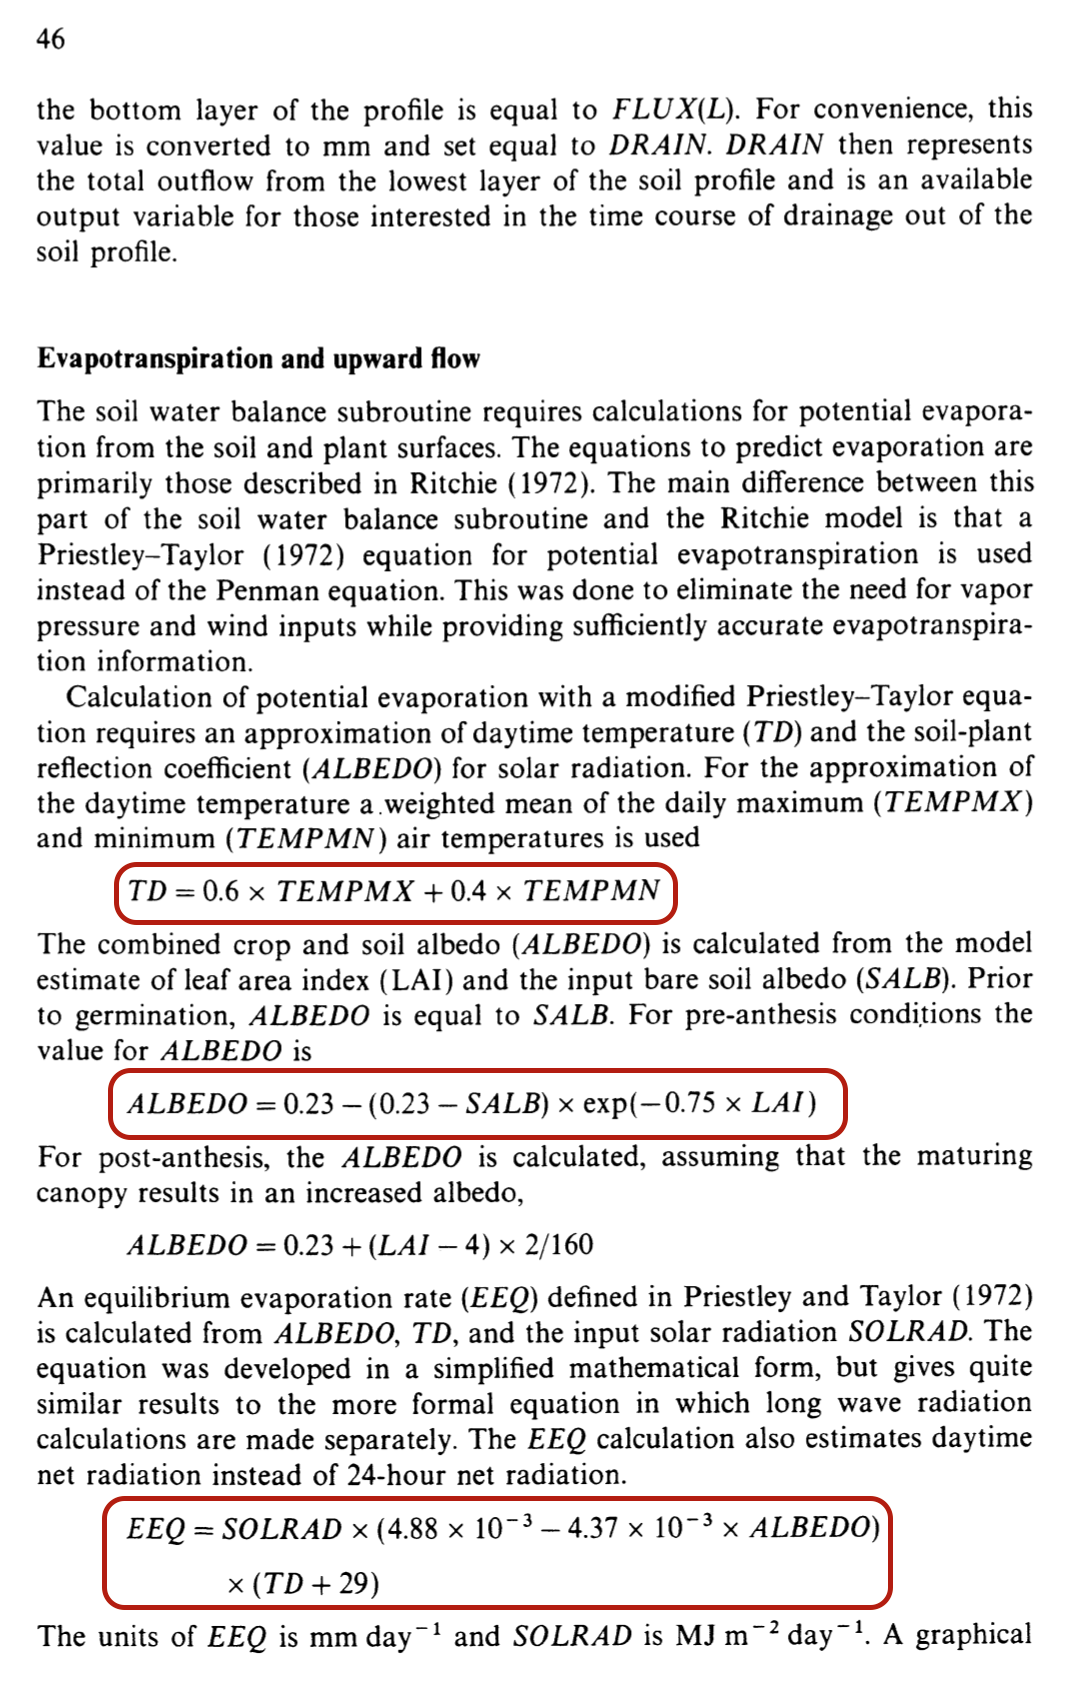
\includegraphics[width=0.90\textwidth]{figs/petpt_equations_example.png}
\caption{Page 46 of the book Understanding Options for Agricultural
Production.\label{fig:uoap-book}}
\end{figure}

% \begin{center}\rule{0.5\linewidth}{\linethickness}\end{center}

\hypertarget{grfn-specification}{%
\section{GrFN Specification}\label{grfn-specification}}

During this phase, significant extensions were made to the GrFN
specification that serves as the central representation between program
analysis (which extracts variables and the network of functions among
them) and model analysis (where the variables and their functional
relationships are treated generally as a probabilistic dynamic systems
model). The extensions include the following.

\hypertarget{identifiers}{%
\subsection{Identifiers}\label{identifiers}}

Prior to this update, a variety of naming conventions were used to
represent source code identifiers (names for program entities such as
variables, constants, functions, etc.), and the disambiguating context
in which they are defined. Identifiers now systematically represent
\emph{namespaces} and program \emph{scope} as part of their definition,
along with their \emph{base name}. The representation of identifiers
includes the following additions and advantages:

\begin{itemize}
\item
  \texttt{\textless{}identifier\_spec\textgreater{}} declarations in
  GrFN associate identifier usage, such as the location within source
  code of where the identifier was declared, as well as ``aliases" (other
  names used to refer to the same program elements). The location of
  identifier use will be used to connect identifiers with source code
  comments and documentation strings. Also, base names, aliases, and
  namespaces will be used as evidence for \emph{grounding} variables to
  model domain concepts.
\item
  Inclusion of namespace and scope context in identifier definitions
  make it possible for program analysis to represent the context of
  Fortran program Modules. This context also provides a consistent
  method for extending source code analysis beyond single source code
  files.
\item
  An \texttt{\textless{}identifier\ string\textgreater{}} provides a
  single human-readable instance of an identifier while consistently
  representing all of its definitional information: namespace, scope,
  and base name. These will be used to denote instances of identifiers
  used in generated GrFN JSON (outside of the identifier declaration
  specs). For example,
\begin{verbatim}
      "CROP_YIELD::UPDATE_EST.loop$1::YIELD_EST"
\end{verbatim}
  is an identifier for a variable name originally given as "YIELD\_EST"
  in source code, but defined in the ``CROP\_YIELD" namespace, and within
  the first loop of the function ``UPDATE\_EST".
\item
  Since identifiers themselves are now defined in terms of structured
  information (namespace, scope, and base name), identifier
  \texttt{\textless{}gensym\textgreater{}}s have been introduced to be
  used as unambiguous standins for identifiers used in generated
  intermediate target Python code.
\end{itemize}

\hypertarget{variable-and-function-naming-conventions}{%
\subsection{Variable and Function Naming
Conventions}\label{variable-and-function-naming-conventions}}

The new systematic representation of namespace and scope rules for
identifiers made it possible to clean up some of the previous ad-hoc
approaches to naming variables and functions. New naming conventions
have been introduced.

\hypertarget{conditions}{%
\subsection{Conditions}\label{conditions}}

The approach to representing program conditions (i.e., ``if statements")
was also updated. When a conditional block in source
code is analyzed, a ``condition" assignment function is introduced that sets the
state of a variable representing the condition, and then one or more
``decision" assignment functions are introduced that represent updates to
other variables depending on the outcome of the condition.

\hypertarget{specification-links}{%
\subsection{Specification Links}\label{specification-links}}

Finally, there was a significant rewrite of the specification
introduction as well as updates throughout to improve readability and
ensure consistency.

The release version of the GrFN specification as of this report is
linked here \href{GrFN_specification_v0.1.m3}{GrFN Specification Version
0.1.m3}. (For the latest development version, see the
\href{https://ml4ai.github.io/delphi/grfn_spec.html}{Delphi
docs page}.)

% \begin{center}\rule{0.5\linewidth}{\linethickness}\end{center}

\hypertarget{program-analysis-for2py}{%
\section{Program Analysis: for2py}\label{program-analysis-for2py}}

Our work in \texttt{for2py} has focused on extending the range of
Fortran language constructs handled. We have implemented support for the
Fortran language constructs listed below. In addition, we have mapped
out the translation of a number of additional Fortran language
constructs and are currently in the process of implementing it.

\hypertarget{fortran-io}{%
\subsection{Fortran I/O}\label{fortran-io}}

Fortran's file and formatted I/O handling mechanisms have been
implemented in \texttt{for2py} so that the pipeline now generates
functionally equivalent Python intermediate representation. This gives
us a way to validate the front-end translation by comparing the
observable behavior of the generated Python code with that of the
original Fortran code. In particular, we have implemented the following:

\begin{enumerate}
\def\labelenumi{\arabic{enumi}.}
\tightlist
\item
  \emph{File Input}: Reading data in from a file. Analogous to Python's
  \emph{read\_line}.
\item
  \emph{File Output}: Writing data to a file in the disk. Analogous to
  Python's \emph{write}.
\item
  \emph{List-Directed Output}: Analogous to Python's \emph{sys.stdout}.
\end{enumerate}

\hypertarget{fortran-modules}{%
\subsection{Fortran Modules}\label{fortran-modules}}

Fortran Modules provide a mechanism for programmers to organize their
code, control visibility of names, and allow code reuse; they are used
extensively in DSSAT as well as other scientific code bases. We have
implemented the conversion of Fortran modules to the \texttt{for2py}
intermediate representation, and validated the translation by confirming
that the resulting Python code has the same behavior as the original
Fortran code.

Our implementation translates each Fortran module into its own Python
file (named 
\emph{\texttt{m\_\textless{}module\_name\textgreater{}.py}}). This has a
number of advantages, among them that it is easy to identify, isolate,
and access the Python code corresponding to each Fortran module, and
also that the Fortran module does not have to be analyzed and translated
to Python more than once. Since Python does not have an explicit
\emph{\texttt{private}} command to limit the visibility of names outside
a given scope, we use Python's
\href{https://docs.python.org/2/tutorial/classes.html\#private-variables-and-class-local-references}{name
mangling} to replicate the behavior of Fortran's \texttt{PRIVATE}
declarations.

We are currently working on implementing the translation of Fortran
modules from the \texttt{for2py} intermediate representation into the GrFN
specification language, where we will make use of the new
\texttt{identifier} and naming conventions.

\hypertarget{open-ended-loops}{%
\subsection{Open-ended Loops}\label{open-ended-loops}}

\texttt{for2py} is able to translate Fortran \texttt{DO-WHILE} loops
into an equivalent Python intermediate represetnation. We are currently
working on implementing the translation of such open-ended loops into
the GrFN specification language.

\hypertarget{arrays}{%
\subsection{Arrays}\label{arrays}}

Fortran arrays differ from Python lists in a number of ways. By default,
Fortran arrays are 1-based, i.e., the first element is at index 1, while
Python lists are 0-based. Fortran arrays can be declared to have lower
bounds different from the default value of 1; this is not true of Python
lists, which always start with index 0. Fortran arrays can be
multi-dimensional, while Python lists themselves are one-dimensional.
Finally, Fortran arrays support operations, such as array constructors,
various sub-array manipulations, array-to-array assignments, etc., that
do not have ready analogs in Python. We have implemented a library that
implements Python objects that support Fortran-like array operations.
Based on this library, we are currently able to translate a wide range
of Fortran array constructs into the \texttt{for2py} intermediate
representation. In particular, we can handle the following Fortran array
features: single- and multidimensional arrays; implicit and explicit
array bounds; and read and write accesses to arrays.

We are currently working on implementing the translation of Fortran
arrays from \texttt{for2py} intermediate representation into the GrFN
specification language.

% \begin{center}\rule{0.5\linewidth}{\linethickness}\end{center}

\hypertarget{text-reading}{%
\section{Text Reading}\label{text-reading}}

\hypertarget{converting-pdf-to-text}{%
\subsection{Converting PDF to text}\label{converting-pdf-to-text}}

As discussed in the previous report, the first task required to perform
automated text reading and information extraction was the conversion of
the source documents from PDF to text. This phase, the team evaluated
several tools on the specific types of documents that are used here
(i.e., scientific papers), and in the end the team chose to use
\href{https://github.com/allenai/science-parse}{science parse} for both
its quick processing of texts as well as the fact that it does a good
job handling section divisions and greek letters. The team integrated
science parse into the text reading pipeline via a Docker container so
that it can be run offline (as a preprocessing step) or online during
the extraction.

\hypertarget{extracting-quantities}{%
\subsection{Extracting quantities}\label{extracting-quantities}}

The team is also utilzing another open-source tool,
\href{https://github.com/kermitt2/grobid-quantities}{grobid-quantities},
which can find and normalize quantities and their units, and even detect
the type of the quantities, e.g., \emph{mass}. The tool finds both
single quantities and intervals, with differing degrees of accuracy. The
grobid-quantities server is run through Docker and the AutoMATES
extraction system converts the extractions into mentions for use in
later rules (i.e., the team's extraction rules can look for a previously
found quantity and attach it to a variable). While grobid-quantities has
allowed the team to begin extracting model information more quickly,
there are limitations to the tool, such as unreliable handling of
unicode and inconsistent intervals. The team has opened several issues
on the Github page for grobid-quanities and will continue to do so. If
nesessary, the extraction of quantities may be moved into the Odin
grammars for full control.

\hypertarget{rule-based-extraction-framework}{%
\subsection{Rule-based extraction
framework}\label{rule-based-extraction-framework}}

The team has begun implementing a lightweight
information extraction framework for use in the ASKE program. The system
incorporates elements of \href{https://github.com/clulab/eidos}{Eidos}
(e.g., the webapp for visualizing extractions, entity finders based on
syntax and the results of grobid-quantities, and the expansion of
entities that participate in relevant events) along with new
\href{http://clulab.cs.arizona.edu/papers/lrec2016-odin.pdf}{Odin}
grammars for identifying, quantifying, and defining variables, as shown
in \autoref{fig:extraction_screenshot}.

\begin{figure}[h]
\centering
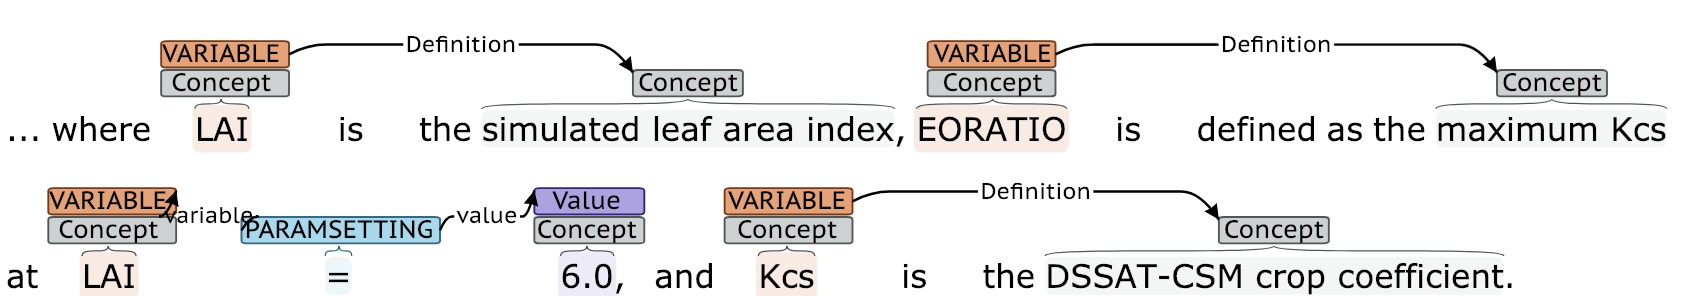
\includegraphics{figs/extractions.png}
\caption{A screenshot of the web-based visualizer showing the results of
the rule-based extraction framework.}
\label{fig:extraction_screenshot}
\end{figure}

This project is fully open-source and has already been utilized and
contributed to by the Georgia Tech ASKE team.

To promote rapid grammar development, the team has developed a framework
for writing unit tests to assess the extraction coverage. Currently,
there are 77 tests written to test the extraction of variables,
definitions, and setting of parameter values, of which 16 pass. This
test-driven approach (in which we first write the tests based on the
desired functionality and then work to ensure they pass) will allow for
quickly increasing rule coverage while ensuring that previous results
are maintained.

\hypertarget{next-steps}{%
\subsection{Next Steps}\label{next-steps}}

The immediate next steps for machine reading are to expand the coverage
of the rules for natural language text and then to begin extracting
information about variables from source code comments. The team will
then create an end-to-end alignment tool to map variables found in code
to the corresponding variable described in natural language.

% \begin{center}\rule{0.5\linewidth}{\linethickness}\end{center}

\hypertarget{equation-detection-and-parsing}{%
\section{Equation Detection and
Parsing}\label{equation-detection-and-parsing}}

\hypertarget{arxiv-bulk-download}{%
\subsection{ArXiv bulk download}\label{arxiv-bulk-download}}

The team has downloaded the complete set of arXiv PDFs and their
corresponding source files from Amazon S3 as described
\href{https://arxiv.org/help/bulk_data_s3}{here}. These will be used for
training and evaluating equation detection and parsing.

\hypertarget{preprocessing-pipeline}{%
\subsection{Preprocessing pipeline}\label{preprocessing-pipeline}}

The team has put together a preprocessing pipeline with the purpose of
preparing the data for training the statistical models for equation
detection.

First, the source files retrieved from arXiv are arranged in a directory
structure where the first directory corresponds to the year and month of
the paper submission (e.g.,\texttt{1810} corresponds to October 2018).
Inside, each paper's source files are stored in a directory named after
the paper's id (e.g., \texttt{1810.04805}).

Then, the file that has the \texttt{\textbackslash{}documentclass}
directive is selected as the main TeX file (see
\href{https://arxiv.org/help/faq/mistakes\#wrongtex}{here} for more
information). Once a main TeX file has been selected, the TeX source is
tokenized and the content of certain environments are collected together
with the environment itself (e.g., the tokens inside the
\texttt{\textbackslash{}begin\{equation\}} and
\texttt{\textbackslash{}end\{equation\}} directives, together with the
label \texttt{equation}).

Currently, the team is focused on processing the TeX code extracted from
the \texttt{equation} environment, while still collecting the code from
other math environments for later use.

The extracted code for each equation is rendered into a standalone
equation image, and then the PDF file for the entire paper is scanned
for this standalone image using
\href{https://docs.opencv.org/4.0.0/df/dfb/group__imgproc__object.html}{template
matching}. The resulting axis-aligned bounding box (AABB) is stored for
the subsequent training of an equation detector.

The team will next work on the preprocessing of the extracted TeX tokens
to provide the equation decoder a more consistent input. At minimum, the
preprocessing will include the removal of superfluous code such as
\texttt{\textbackslash{}label\{\}} directives, the normalization of
certain LaTeX expressions (e.g., arbitrary ordering of super and
sub-scripts in equations), and expanding user-defined macros.

\hypertarget{data-driven-analysis-of-preamble-to-inform-template-design}{%
\subsubsection{Data driven analysis of preamble to inform template
design}\label{data-driven-analysis-of-preamble-to-inform-template-design}}

The team has conducted an analysis on a sample of 1600 of the arXiv
retrieved sources to inform the design of the templates used to render
standalone equation images. The purpose of this analysis is the
identification of the math environments and TeX packages that are most
commonly used for the writing of math in academic papers, which
will help the team assemble a
template that (a) has broad coverage (i.e., can make the most use of the
training data) and (b) is minimal (i.e., will be faster to run and will
have fewer conflicts).

The analysis shows that the most commonly used math environments (in
order) are: \texttt{equation}, \texttt{align}, and
\texttt{\textbackslash{}{[}\ \textbackslash{}{]}}. While the team
currently handles the \texttt{equation} environment (40\% of the
equations found), the pipeline will be extended to accomodate the other
two as well. In terms of the preamble packages related to math
rendering, both \texttt{amsmath} and \texttt{amssymb} occurred in over
70\% of the main files, and the next most common package
(\texttt{amsfonts}) occurred in only 35\% of the main files.
Accordingly, the initial template for rendering the standalone equations
contains those two most prevalent packages for now, with the option to
extend as needed in the future.

\hypertarget{deploying-im2markup-on-uofa-hpc}{%
\subsection{\texorpdfstring{Deploying \texttt{im2markup} on UofA
HPC}{Deploying im2markup on UofA HPC}}\label{deploying-im2markup-on-uofa-hpc}}

The team has also built a
\href{https://www.sylabs.io/guides/3.0/user-guide/}{singularity
container} with the lua and Python libraries required to run
\href{https://github.com/harvardnlp/im2markup}{im2markup}. This will
allow for rapid development of the equation decoding system.

% \begin{center}\rule{0.5\linewidth}{\linethickness}\end{center}

\hypertarget{model-analysis}{%
\section{Model Analysis}\label{model-analysis}}

A key goal of model analysis is to enable comparison of models that
describe the underlying target domain. When the models overlap, they
share some variables, but likely not others. The first task in comparing
GrFN function networks is to identify where the models overlap. We first
review the team's work on automating function network comparison, and
then present some initial results investigating the complexity of
running sensitivity analysis, which in turn is informing our next
approaches to scaling sensitivity analysis.

\hypertarget{automated-function-network-comparison}{%
\subsection{Automated function network
comparison}\label{automated-function-network-comparison}}

During this phase, the team developed an algorithm to identify the
shared portion of two function networks. As a working example, we show
what the algorithm identifies as the overlapping subnetworks of two
evapotranspiration models in the DSSAT system: ASCE and
Priestley-Taylor.  Figures~\ref{fig:pt}~\&~\ref{fig:asce} show a graphical
representation of the shared portions of these two models, which are
identified by a network property that we refer to as a \emph{Forward
Influence Blanket} (FIB). In the following section we will formally
define the structure of a FIB and its role in model analysis.

% \begin{center}\rule{0.5\linewidth}{\linethickness}\end{center}

\begin{figure}
\centering
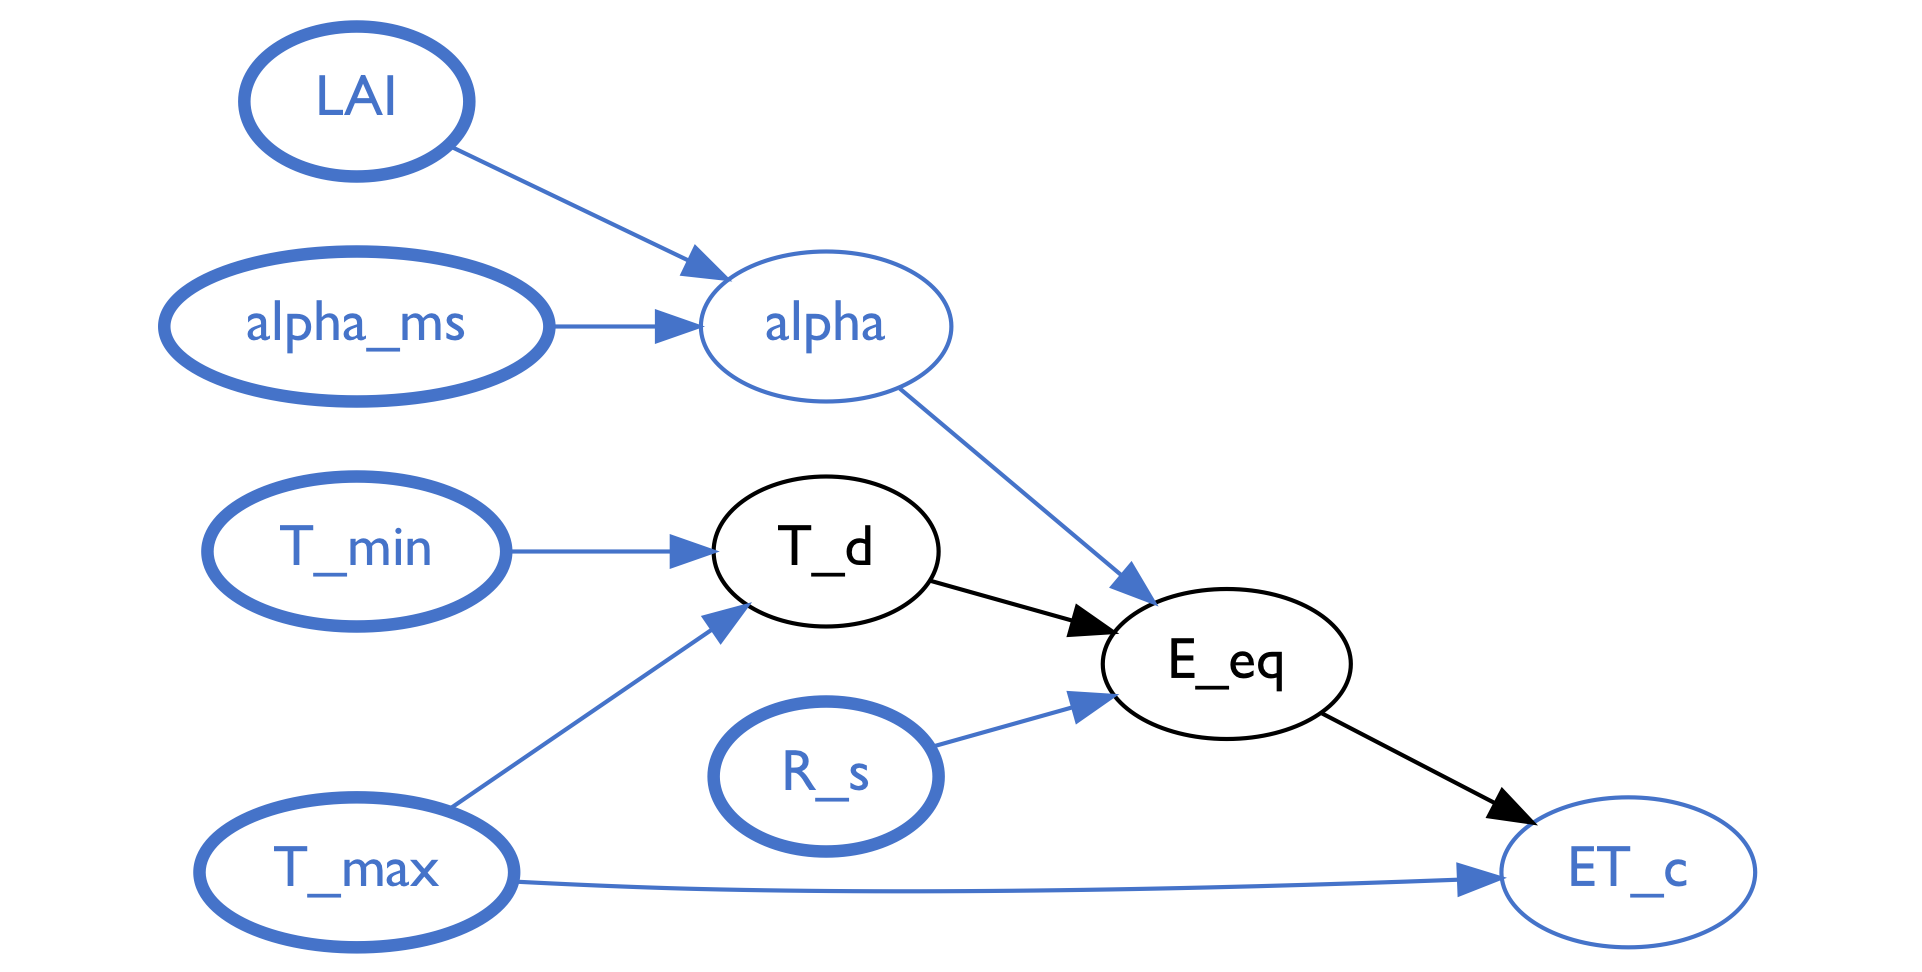
\includegraphics{figs/full-pt-cmb.png}
\caption{Representation of the subnetwork within the Priestley-Taylor
model identified by the Forward Influence Blanket that intersects with
the ASCE model.\label{fig:pt}}
\end{figure}

% \begin{center}\rule{0.5\linewidth}{\linethickness}\end{center}

\begin{figure}
\centering
\includegraphics{figs/full-asce-cmb.png}
\caption{Representation of the subnetwork within the ASCE model
identified by the Forward Influence Blanket that intersects with the
Priestley-Taylor model.\label{fig:asce}}
\end{figure}

% \begin{center}\rule{0.5\linewidth}{\linethickness}\end{center}

\hypertarget{identifying-the-forward-influence-blanket-fib}{%
\subsection{Identifying the Forward Influence Blanket
(FIB)}\label{identifying-the-forward-influence-blanket-fib}}

Drawing a loose analogy to a
\href{https://en.wikipedia.org/wiki/Markov_blanket}{Markov Blanket}, a
\emph{Forward Influence Blanket} identifies the variables that are
shared between two function networks, along with the non-shared
variables that are involved in any functional relationships that are
along the directed paths between the shared variables. The FIB gets its
name because we are analyzing the \emph{influence} that variables have
on one another in a directed (\emph{forward} from input to output)
network, and the \emph{blanket} identifies minimal subset of such
influences shared between the two networks.

Figures~\ref{fig:pt}~\&~\ref{fig:asce} depict 
(through node coloring) the portions of the
function networks for the two models identified as overlapping. The
nodes in the graphs represent variables, the directed arcs indicate
directed functional relationships (the variable at the tail is an input,
the variable at the head is the output variable that is a function of
the input), and the nodes are color-coded to provide a visual depiction
of different relationships with respect to the FIB.

Consider Figure~\ref{fig:asce}, depicting the ASCE function network. All the
blue nodes in the network represent variables that are also found in the
Priestly-Taylor model. The blue nodes with thicker lines represent
variables that play ``input" roles in both of the overlapping
subnetworks: they are shared and do not have any parents that are also
in the subnetworks.

Next, between the blue nodes and along the directed paths from the
``inputs" to the output nodes, are black nodes that represent variables
that are not shared between the two models; these indicate intermediate
values that may represent differences in the functional relationships
between the inputs and outputs of the subnetwork. Determining what the
functional differences may be is the subject of the next phase,
sensitivity analysis, described in the next section.

In Figure~\ref{fig:pt}, depicting the Priestley-Taylor function network,
all of the black nodes are between blue nodes. In fact, there are no
other nodes or edges that are not colored blue and black. This means the
inputs and outputs of the Priestley-Taylor network are ``contained
within" the ASCE network while there are some differences in the
computation between the inputs and outputs (the black nodes).

In the ASCE network, however, there are a number of additional nodes:
the green colored nodes identify the variables that have directed
influence on the computations along the paths from inputs to outputs,
although they are \emph{not} shared between the networks. If one is
interested in directly comparing the subnetworks to each other, the
states of the green variables may affect the input-to-output
relationships.

Finally, the orange nodes in Figure~\ref{fig:asce} represent all of the variables in the ASCE
model that are not shared by the Priestley-Taylor model and cannot
directly affect the functional relationships between the shared inputs
and outputs without either first passing through a blue or green node.
It is in this sense that the green and blue nodes together form the
\textbf{blanket} that isolates the functional relationships between the
inputs and outputs that are shared between the two networks. If we
understand the functional relationships among the blue and green nodes,
then we can separately consider how the orange nodes affect each other,
and their relationships are only relevant to describing the behavior of
the ASCE model. This provides a nice way of factoring the overall
analysis into separate analysis tasks.

Having identified the FIB, with the blue and green nodes constituting
all of the inputs that can eventually affect the output(s), we can now
turn to analyze the functional relationship between inputs and outputs,
including the sensitivity of output variables to input variable values.

\hypertarget{sensitivity-index-discovery}{%
\subsection{Sensitivity index
discovery}\label{sensitivity-index-discovery}}

In our previous report we demonstrated the ability to automatically
conduct sensitivity analysis on the inputs to an extracted function
network. The method we presented involved three steps to fully conduct a
sensitivity analysis of a given function \emph{f}:

\begin{enumerate}
\def\labelenumi{\arabic{enumi}.}
\tightlist
\item
  Take \emph{N} samples from the input space of \emph{f} using
  \href{https://en.wikipedia.org/wiki/Variance-based_sensitivity_analysis}{Saltelli
  sampling}
\item
  Evaluate each of the \emph{N} samples on \emph{f} to form the set
  \emph{E}
\item
  Perform
  \href{https://en.wikipedia.org/wiki/Variance-based_sensitivity_analysis}{Sobol
  analysis} on \emph{E}
\item
  Recover the \(S_1\), \(S_2\), and \(S_T\) sensitivity indices
\end{enumerate}

\noindent This method has been successful in retrieving all the information we
needed in order to determine which inputs account for the most
uncertainty in model output. Since the last report, the team has begun
investigating how the runtime of sensitivity analysis is affected by
varying the sample size \emph{N} or the size of the input space (number
of input variables) of function \emph{f}. The purpose of this study is
to understand which aspects of models contribute to the complexity of
sensitivity analysis. Below we present and discuss plots (Figures~\ref{fig:sa_samples}~\&~\ref{fig:sa_inputs}) of runtime as a
function of the sample size and number of variables. For each of these
graphs the red line shows the runtime for the entirety of sensitivity
analysis and the blue line shows the runtime of part (3) of the
analysis. All run times are in units of seconds.

\hypertarget{runtime-as-a-function-of-sample-size}{%
\paragraph{Runtime as a function of sample
size}\label{runtime-as-a-function-of-sample-size}}

As models become more complex we expect that we will need to increase
the number of samples taken and evaluated in order to achieve comparable
accuracy in sensitivity index estimation during sensitivity analysis.
Because of this, we determined that we needed to empirically inspect the
runtime of sensitivity analysis as the number of samples increases. 
In Figures~\ref{fig:sa_samples}, we can see that the increase in runtime as the number
of samples increases is nearly linear (with slight super-linear trend),
both for the entirety of sensitivity analysis and for the Sobol portion
of sensitivity analysis. This result is encouraging because it suggests
that as long as we maintain only a linear increase in the number of
samples required to conduct sensitivity analysis on our larger models
then we should not see a runtime increase that would render sensitivity
analysis intractable.

% \begin{center}\rule{0.5\linewidth}{\linethickness}\end{center}

\begin{figure}
\centering
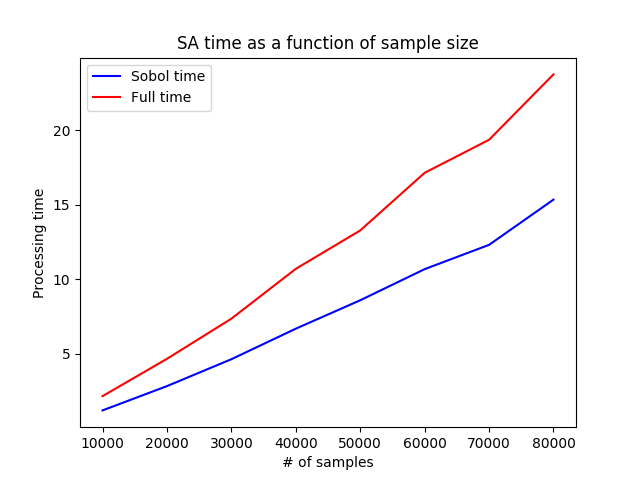
\includegraphics{figs/sa_samples_vs_runtime.png}
\caption{Plot of the increase in runtime for our Sobol analysis method
as sample size increases. The blue line depicts the increase in runtime
for the Sobol algorithm and the red line depicts the runtime for the
total program.\label{fig:sa_samples}}
\end{figure}

% \begin{center}\rule{0.5\linewidth}{\linethickness}\end{center}

\hypertarget{runtime-as-a-function-of-the-number-of-input-variables}{%
\paragraph{Runtime as a function of the number of input
variables}\label{runtime-as-a-function-of-the-number-of-input-variables}}

We are also exploring the impact of increasing the number of input
variables considered during an analysis on overall runtime. As expected,
Figure~\ref{fig:sa_inputs} does show that the runtime for the Sobol portion of
sensitivity analysis increases super-linearly as the number of input
variables increases. To address this, we are currently exploring several
ways to reduce the number of inputs analyzed at one time. One strategy
already described above, motivating the FIB analysis, is to identify
modular components of the function network with fewer inputs that can be
analyzed independently. We are also exploring doing this at the level of
performing sensitivity analysis one function at a time, and then
composing the results.

% \begin{center}\rule{0.5\linewidth}{\linethickness}\end{center}

\begin{figure}
\centering
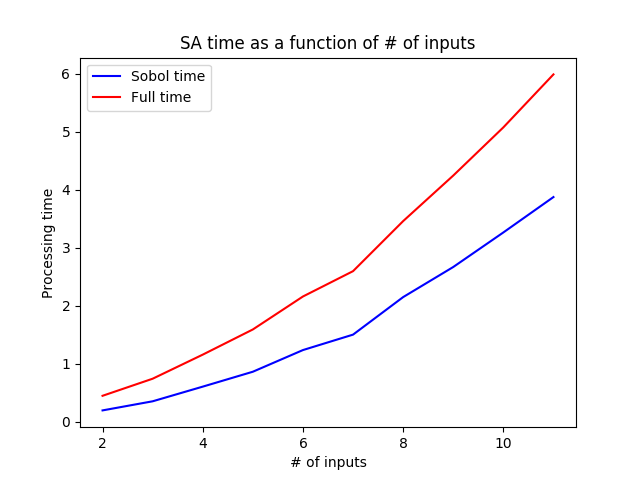
\includegraphics{figs/sa_inputs_vs_runtime.png}
\caption{Plot of the increase in runtime for the Sobol analysis method
given an increase in number of inputs for the function under analysis.
The blue line depicts the increase in runtime for the Sobol algorithm
and the red line depicts the runtime for the total program.\label{fig:sa_inputs}}
\end{figure}

% \begin{center}\rule{0.5\linewidth}{\linethickness}\end{center}

\hypertarget{code-summarization}{%
\section{Code Summarization}\label{code-summarization}}

During this phase, the team began exploring an encoder/decoder
neural network model for code summary generation. Initial results
demonstrated that the model was not able to acquire enough signal to
adequately generate summarizations for source code. In
response, the team developed the following three tasks to improve the
model.

\begin{itemize}
\item
  The first task involved reassessing the quality of the code/docstring
  training corpus to see if there are avoidable sources of error in the
  corpus and to attempt to gather more data.
\item
  The second task involved trying different approaches to the
  code/docstring embeddings by investigating the vocabulary size (too
  many vocabulary items can lead to data sparsity) and possible methods
  for reducing it.
\item
  The third task involved creating a model for a simpler task
  (classification) that has the same form as the model for our
  generation task but can be used to directly assess the embedding
  representation quality.
\end{itemize}

In the following three sections we will outline the progress we have
made on these three tasks.

\hypertarget{progress-on-codedocstring-corpus}{%
\subsection{Progress on code/docstring
corpus}\label{progress-on-codedocstring-corpus}}

The team was able to increase the size of our overall code/docstring
corpus by indexing more Python packages to identify additional Python
functions that have PEP-style descriptive docstrings. We were able to
index additional Python packages from the following lists of packages:
the
\href{https://docs.anaconda.com/anaconda/packages/py3.6_osx-64/}{anaconda
distribution}, the
\href{https://github.com/vinta/awesome-python}{awesome-python} list, and
the list of all available
\href{http://scikits.appspot.com/scikits}{SciKit packages}. In total, we
increased the amount of Python packages that we are searching for
code/docstring pairs from 24 to 1132.

\begin{figure}[h]
\centering
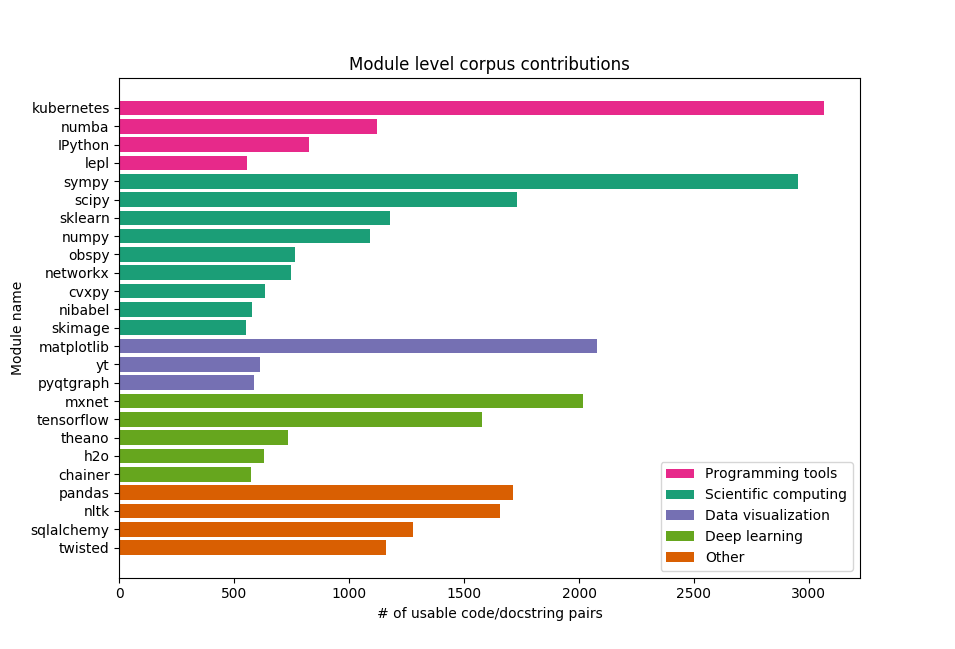
\includegraphics{figs/module_corpus_contributions.png}
\caption{Graphical view of the amount of usable code/docstring pairs
each Python module has added to our code-summarization corpus (only the
25 modules with the largest amount of usable pairs are shown). Modules
are color-coded according to the type of code most likely to be found in
the module.\label{fig:sum_corpus}}
\end{figure}

From these packages, we have extracted code/docstring pairs, increasing
our corpus from approximately 22,000 examples to approximately 82,000.
Figure~\ref{fig:sum_corpus} summarizes the styles of code-bases and their
relative contributions to our corpus.

% \begin{center}\rule{0.5\linewidth}{\linethickness}\end{center}

% Pairs each python module has added to our code-summarization corpus (only the 25 modules with the largest amount of usable pairs are shown) Modules are color-coded according to the type of code most likely to be found in the module.

% \begin{center}\rule{0.5\linewidth}{\linethickness}\end{center}

\hypertarget{progress-on-code-embeddings}{%
\subsection{Progress on code
embeddings}\label{progress-on-code-embeddings}}

The performance of neural networks has been found to strongly depend on
the quality of the embedding model used to represent the data. One of
the biggest struggles for any embedding is to ensure that enough
examples are present for every token you wish to embed. Without a large
number of examples, the embedding space cannot create meaningful
embeddings for corresponding tokens. In the case of creating embeddings
for code, it is likely that the names of functions are going to
be some of the most important tokens to embed. Unfortunately, these
are also the most infrequent, if each unique name is treated as a single
token. From our original dataset of 22,000 examples, we had roughly
53,000 unique tokens in the code portion of our corpus. The vast
majority of these were function or variable names that occurred fewer
than five times each, not nearly enough to be able to establish useful
embeddings that capture the type of semantic information carried in
function or variable names.

To address this issue, we split function and variable names into
sub-components using \texttt{snake\_case} and \texttt{camelCase} rules,
to extract the repeated mentions of name that occur as parts of function
and variable names. Some examples of the tokenized forms of function
names found in our corpus before and after the transformation are
provided in the following table.

\begin{longtable}[]{@{}ll@{}}
\toprule
Original tokenization & Split-name tokenization\tabularnewline
\midrule
\endhead
\texttt{compute\_ldap\_message\_size} &
\texttt{\textless{}BoN\textgreater{}\ compute\ ldap\ message\ size\ \textless{}EoN\textgreater{}}\tabularnewline
\texttt{getComponentByPosition} &
\texttt{\textless{}BoN\textgreater{}\ get\ Component\ By\ Position\ \textless{}EoN\textgreater{}}\tabularnewline
\texttt{fromOpenSSLCipherString} &
\texttt{\textless{}BoN\textgreater{}\ from\ Open\ SSL\ Cipher\ String\ \textless{}EoN\textgreater{}}\tabularnewline
\texttt{fromISO8601} &
\texttt{\textless{}BoN\textgreater{}\ from\ ISO\ 8601\ \textless{}EoN\textgreater{}}\tabularnewline
\bottomrule
\end{longtable}

Splitting functions/variable names in this way decreased our code
vocabulary size from roughly 53,000 to roughly 16,000 unique tokens
while also lowering the number of tokens that appear fewer than five
times from roughly 35,000 to roughly 5,000.

\hypertarget{docstring-classification-task}{%
\subsection{Docstring classification
task}\label{docstring-classification-task}}

One of the difficulties with generation tasks is being able to tell
whether a model has enough signal from the data to be able to
generate affectively.
In order to evaluate whether our dataset provides enough signal for our
generation task, we have designed a separate classification task in
which the classifier is presented with a code and docstring pair and
must predict whether the docstring describes the code, which we
approximate by using the docstrings associated with code blocks in our
corpus. In the following sections, we describe the classifier,
present the two classification datasets we are using and some
preliminary results, followed by a discussion of the next steps for using
these methods to improve the code summary generation model.

\hypertarget{baseline-neural-model-description}{%
\paragraph{Baseline neural model
description}\label{baseline-neural-model-description}}

Our initial classification model is a simplification from the model we
originally planned to use for generation. The model first embeds a code
sequence and a docstring using our pretrained code 
and docstring embeddings. The two embedded sequences
are each fed into their own respective
\href{https://pdfs.semanticscholar.org/4b80/89bc9b49f84de43acc2eb8900035f7d492b2.pdf}{Bi-LSTM
recurrent network}. The final hidden state outputs from these networks
are then concatenated and fed into a deep feed-forward neural network
that produces a binary classification of whether the docstring is
correctly paired with the provided function.

Our rationale for simplifying the model used for classification is that
we are currently testing to see if our data is providing enough signal
to aid in classification. Once we verify that we do have enough signal
to allow for decent classification results, we will increase the
complexity of the model. It is important to note that since the main purpose of the
classification model is to test the fitness of our data for generation,
we cannot add any docstring specific information to the classification
model, since such information would not be present during docstring
generation.

\hypertarget{random-draw-and-challenge-dataset-description}{%
\paragraph{Random-draw and challenge dataset
description}\label{random-draw-and-challenge-dataset-description}}

We have constructed two different datasets from our code/docstring
corpus that we will use to test the classification model. The corpus
itself only provides positive examples of docstrings paired with code
blocks, so in order to create negative examples, we use a common
practice in NLP known as \emph{negative sampling} to match code blocks
with docstrings other than their correct docstring. This creates
instances for our classifier to correctly label as mismatched pairs. We
have done this with both of our datasets.

For our first dataset, we use uniform random sampling to select our
negative examples. We named this the ``random-draw'' dataset. We
anticipate that this dataset will be easier to obtain good performance
as uniform random sampling is likely to pair docstrings with code that
is completely unrelated. This dataset is used for the earliest phases of
experimentation with our classifier as we are expected to have better
chance of training success. Once we determine that our classifier can do
reasonably well on the random-draw dataset we will move on to testing
our model on our second dataset.

The second dataset uses lexical overlap between the true docstring for a
code block and the other candidate docstrings to select a candidate that
has the highest lexical overlap with the true docstring (i.e., shares
many of the same terms), but is not the correct pairing. This is called
the ``challenge'' dataset, as now the ``mismatch'' pairings are much
more likely to be close but still not correct. This allows us to
rigorously test our classifier's ability to correctly identify whether a
code/docstring pair is mismatched. To build the dataset, we use
\href{http://lucene.apache.org/}{Apache Lucene} to index and query our
set of docstrings. The following table shows five docstrings with their
negative example docstring of highest lexical overlap is provided in the
table below.

\begin{longtable}[]{@{}lll@{}}
\toprule
\begin{minipage}[b]{0.31\columnwidth}\raggedright
Module paths (source, negative)\strut
\end{minipage} & \begin{minipage}[b]{0.31\columnwidth}\raggedright
Source docstring\strut
\end{minipage} & \begin{minipage}[b]{0.29\columnwidth}\raggedright
Best negative example\strut
\end{minipage}\tabularnewline
\midrule
\endhead
\begin{minipage}[t]{0.31\columnwidth}\raggedright
{\footnotesize \texttt{kubernetes.client.api}\\ \texttt{tabpy.client.rest}}\strut
\end{minipage} & \begin{minipage}[t]{0.31\columnwidth}\raggedright
Builds a JSON POST object\strut
\end{minipage} & \begin{minipage}[t]{0.29\columnwidth}\raggedright
Issues a POST request to the URL with the data specified . Returns an
object that is parsed from the response JSON\strut
\end{minipage}\tabularnewline
\begin{minipage}[t]{0.31\columnwidth}\raggedright
{\footnotesize \texttt{sympy.ntheory.multinomial}\\ \texttt{statsmodels.iolib.table}}\strut
\end{minipage} & \begin{minipage}[t]{0.31\columnwidth}\raggedright
Return a list of binomial coefficients as rows of the Pascal's
triangle\strut
\end{minipage} & \begin{minipage}[t]{0.29\columnwidth}\raggedright
Return list of Row , the raw data as rows of cells\strut
\end{minipage}\tabularnewline
\begin{minipage}[t]{0.31\columnwidth}\raggedright
{\footnotesize \texttt{matplotlib.image}\\ \texttt{PIL.image}}\strut
\end{minipage} & \begin{minipage}[t]{0.31\columnwidth}\raggedright
Set the grid for the pixel centers , and the pixel values\strut
\end{minipage} & \begin{minipage}[t]{0.29\columnwidth}\raggedright
Gets the the minimum and maximum pixel values for each band in the
image\strut
\end{minipage}\tabularnewline
\begin{minipage}[t]{0.31\columnwidth}\raggedright
{\footnotesize \texttt{mxnet.model}\\ \texttt{tensorflow.engine.training}}\strut
\end{minipage} & \begin{minipage}[t]{0.31\columnwidth}\raggedright
Run the model given an input and calculate the score as assessed by an
evaluation metric\strut
\end{minipage} & \begin{minipage}[t]{0.29\columnwidth}\raggedright
Sets the metric attributes on the model for the given output\strut
\end{minipage}\tabularnewline
\begin{minipage}[t]{0.31\columnwidth}\raggedright
{\footnotesize \texttt{twisted.internet.tcp}\\ \texttt{gevent.server}}\strut
\end{minipage} & \begin{minipage}[t]{0.31\columnwidth}\raggedright
Create and bind my socket , and begin listening on it\strut
\end{minipage} & \begin{minipage}[t]{0.29\columnwidth}\raggedright
A shortcut to create a TCP socket , bind it and put it into listening
state\strut
\end{minipage}\tabularnewline
\bottomrule
\end{longtable}

\hypertarget{initial-classification-results}{%
\paragraph{Initial classification
results}\label{initial-classification-results}}

We have trained and evaluated our baseline model on the random-draw
dataset that was generated by our original corpus (22,000 pairs). After
processing over our training set for 35 epochs, our validation set
accuracy was 80\%, a result that we are very excited about!

\hypertarget{next-steps-1}{%
\paragraph{Next steps}\label{next-steps-1}}

Now that we have increased our corpus size and created our challenge
dataset, our immediate next task is to re-evaluate our baseline model on
both the random-draw dataset and challenge dataset to see how the
changes to our code/docstring corpus affect our performance on our two
datasets.

Pending encouraging results on the above experiments, we will begin
increasing the complexity of the model by adding character embeddings
for the code/docstring tokens. We also plan to add attention layers to
the LSTM output from the code and docstring LSTMs that add attention on
the alternate sequence respectively. If the results from the above
experiments are not as good as we hoped then we will also investigate
adding more docstring data to our docstring embeddings from large online
documenation repositories such as
\href{https://readthedocs.org/}{ReadTheDocs} to improve the signal from
our docstring sequences.

\end{document}
